\documentclass[border=4pt]{standalone}
\usepackage{tikz}
\usepackage{zx-calculus}
\begin{document}
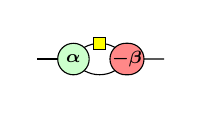
\begin{tikzpicture}[x=1cm, y=1cm]
  \node at (0.83,-0.26) {\pgfinterruptpicture%
  \begin{ZX}
  \zxN{} \rar &[\zxwCol] \zxZ{\alpha} \ar[r,o',H] \ar[r,o.] &[\zxHCol] \zxX-{\beta} \rar &[\zxwCol] \zxN{}
  \end{ZX}%
  \endpgfinterruptpicture};
\end{tikzpicture}
\end{document}
